\documentclass{article}

\usepackage[final]{neurips_2020}
\usepackage{amsmath, amssymb}
\usepackage{graphicx}
\usepackage{booktabs}
\usepackage{hyperref}
\usepackage{caption}
\usepackage{subcaption}
\usepackage{graphicx}
\usepackage{hyperref}
\usepackage{natbib}
\usepackage{geometry}
\geometry{margin=1in}
\usepackage{microtype}
\usepackage{enumitem}
\usepackage{authblk}
\usepackage{cleveref}
\usepackage[final]{neurips_2020}
\usepackage[utf8]{inputenc}
\usepackage[T1]{fontenc}
\usepackage{hyperref}
\usepackage{url}
\usepackage{booktabs}
\usepackage{amsfonts, amsmath, amsthm}
\usepackage{nicefrac}
\usepackage{microtype}
\usepackage{graphicx}
\usepackage{subcaption}
\usepackage{algorithm}
\usepackage{algorithmic}
\usepackage{bbm}

\title{Spectral Flattening for Kernel SVMs:\\
A Study of Covariance-Adaptive Kernels on Synthetic and Pretrained Feature Spaces}

\author{
Elise Wolf\\
ENSAE Paris\\
\texttt{elisemarie.wolf@ensae.fr}
}

\begin{document}

\maketitle

\begin{abstract}

Kernel methods such as Support Vector Machines rely on distances in feature space, and when features are anisotropic, Euclidean distances are dominated by high-variance directions. Modern classifiers often operate on high-dimensional features from pretrained deep networks, which are highly anisotropic, meaning that discriminative information may be concentrated in a few high-variance directions.  

We study \emph{spectral flattening}, a simple covariance-adaptive transformation parametrized by $\beta \in [0, 0.5]$, interpolating between isotropic RBF kernels ($\beta=0$) and the Mahalanobis kernels ($\beta=0.5$). Synthetic experiments confirm that flattening successfully amplifies low-variance signal, reducing condition numbers and improving accuracy dramatically (+38.4\%).  

However, evaluation on real-world datasets (CUB-200-2011, Stanford Cars) with pretrained ResNet50, ViT, and ConvNeXt features reveals minimal or negative gains. Discriminative information in these features resides primarily in high-variance dimensions, causing flattening to amplify noise rather than signal.  

Our results precisely define the boundary of applicability, namely spectral flattening is effective when low-variance directions carry meaningful signal, such as in synthetic, unsupervised, generative, or domain-shifted embeddings, but offers limited utility for standard pretrained features.
\end{abstract}

\section{Introduction}

Kernel methods occupy a unique position in machine learning. On the one hand, they are among the most theoretically well-understood tools in the field, with guarantees stemming from convex optimization. On the other hand, they remain competitive in practice, particularly in settings with limited data, high-dimensional features, or strong inductive biases \cite{scholkopf2002learning}.

Among kernel methods, the Support Vector Machine (SVMs) with a radial basis function (RBF) kernel is especially popular due to its universal approximation properties and simplicity. Classification decisions in the RBF kernel are based on distances between points in feature space. Yet this apparent simplicity hides a crucial assumption—namely, that Euclidean distance in feature space is a meaningful measure of similarity.

In modern machine learning pipelines, kernel classifiers are rarely applied to raw data. Instead, they are often trained on representations extracted from deep neural networks pretrained on large-scale datasets such as ImageNet. While these representations are empirically powerful, recent work has shown that they possess variance concentrated in few principal directions, referred to as highly anisotropic covariance structure, with a small number of principal components explaining the vast majority of variance \cite{papyan2020prevalence}. This raises the question of how the RBF kernel behaves on such anisotropic feature spaces.

This project is motivated by the observation that the standard RBF kernel implicitly emphasizes high-variance directions, potentially suppressing informative but low-variance features. Spectral flattening is a principled attempt to correct this imbalance by explicitly incorporating the empirical covariance of the data into the kernel definition. While appealing in theory, its practical behavior on modern pretrained representations is not yet understood \cite{papyan2020prevalence}.

The idea of covariance-aware kernel design has appeared in several contexts. In one-class classification, Khan et al.~\cite{khan2014covariance} observed that outliers often differ from normal data along low-variance directions and proposed covariance-guided kernels to emphasize such structure. Tax and Juszczak~\cite{tax2002kernel} explored kernel whitening for anomaly detection, effectively corresponding to the fully whitened case $\beta=0.5$. More generally, Mahalanobis kernels normalize distances by the inverse covariance and have long been recognized as a principled alternative to Euclidean distance.

We aim to develop kernel geometry, variance weighting, and feature anisotropy to a nuanced understanding of why spectral flattening succeeds in controlled settings yet largely fails on real pretrained features.

\section{Background and Motivation}

To understand the motivation behind spectral flattening, it is essential to revisit how kernel SVMs operate geometrically.

The Gaussian RBF kernel between two feature vectors $x, x' \in \mathbb{R}^d$ is defined as
\[
k(x, x') = \exp\left(-\frac{\|x - x'\|^2}{2\sigma^2}\right).
\]
This kernel assigns high similarity to points that are close in Euclidean distance and rapidly decays as distance increases. When used in an SVM, classification decisions are therefore governed by pairwise distances between feature vectors.

Crucially, Euclidean distance is not invariant to feature scaling. If one coordinate exhibits substantially larger variance than another, it will dominate the distance computation, irrespective of whether that coordinate is informative for the classification task. In high-dimensional representations learned by modern neural networks, this effect becomes extreme. Empirical feature covariances are often highly anisotropic, with a small number of principal components accounting for the vast majority of variance. As a result, the RBF kernel effectively measures similarity almost exclusively along these dominant directions.

From a geometric perspective, this implies that low-variance directions contribute negligibly to pairwise distances. Even if two classes differ systematically along such directions, their influence on the kernel similarity is smaller than the noise in high-variance dimensions. The kernel thus implicitly assumes that variance correlates with discriminative importance, which is an assumption that is rarely stated explicitly, but embedded in the use of Euclidean distance. This observation motivates to modify the kernel geometry such that low-variance directions receive greater emphasis, without fully discarding the stabilizing effect of variance-based weighting.

A classical approach to correcting variance imbalance in kernel methods is to replace the Euclidean distance by a Mahalanobis distance induced by the inverse data covariance. Let $\Sigma \in \mathbb{R}^{d \times d}$ denote the empirical covariance matrix of the feature vectors, assumed to be symmetric and positive definite. The Mahalanobis kernel is defined as
\[
k_{\text{Mah}}(x, x') 
= \exp\left(
    -\frac{(x - x')^\top \Sigma^{-1} (x - x')}{2\sigma^2}
\right).
\]
This kernel is equivalent to applying a whitening transformation to the features prior to computing the standard RBF kernel. While this transformation eliminates spectral anisotropy entirely, it enforces equal weighting across all directions, including those dominated by noise, which can lead to degraded generalization performance.

Spectral flattening generalizes this idea by introducing a continuous family of covariance-adaptive transformations that interpolate between the standard RBF kernel and the fully whitened kernel. Let the eigendecomposition of the empirical covariance matrix be given by
\[
\Sigma = U \Lambda U^\top,
\]
where $U$ is an orthogonal matrix of eigenvectors and $\Lambda = \mathrm{diag}(\lambda_1, \ldots, \lambda_d)$ is a diagonal matrix of eigenvalues ordered such that $\lambda_1 \geq \lambda_2 \geq \dots \geq \lambda_d > 0$.

For a parameter $\beta \in [0, 0.5]$, spectral flattening defines the linear transformation
\[
T_\beta := U \Lambda^{-\beta} U^\top.
\]
Applying this transformation to the feature vectors yields the covariance-adaptive RBF kernel
\[
k_\beta(x, x') 
= \exp\left(
    -\frac{\|T_\beta (x - x')\|^2}{2\sigma^2}
\right).
\]

The effect of spectral flattening on the feature geometry can be characterized analytically. The covariance matrix of the transformed features is given by
\[
\Sigma_\beta 
= T_\beta \Sigma T_\beta^\top
= U \Lambda^{1 - 2\beta} U^\top.
\]
Hence, the eigenvalues of $\Sigma_\beta$ are $\lambda_i^{1 - 2\beta}$ for $i = 1, \ldots, d$. It follows immediately that the \emph{condition number} 
\[
\kappa(\Sigma_\beta) = \left(\frac{\lambda_{\max}}{\lambda_{\min}}\right)^{1-2\beta}= \kappa(\Sigma)^{1 - 2\beta},
\]
as the ratio of its largest to smallest eigenvalue of the transformed covariance, measuring the degree of spectral anisotropy, satisfies and therefore decreases monotonically as monotonically as $\beta$ increases from 0 to 0.5.

This formulation explicitly recovers several important special cases. For $\beta = 0$, $T_\beta = I$ and the standard isotropic RBF kernel is obtained. For $\beta = 0.5$, $T_\beta = \Sigma^{-1/2}$ and the kernel reduces exactly to the Mahalanobis kernel defined above. Intermediate values of $\beta$ interpolate smoothly between these two extremes by partially compensating for spectral anisotropy.

In addition to reducing the condition number, spectral flattening increases the \emph{effective rank} of the covariance matrix, which measures how uniformly variance is distributed across eigenvalues, with higher values indicating more balanced spectral energy. This redistributes variance more evenly across dimensions, making the induced kernel geometry progressively less dominated by a small number of high-variance principal components. 

To make the effect of spectral flattening concrete, we visualize it on a 2D binary classification problem with diagonal covariance $\Sigma = \text{diag}(100, 1)$ (condition number $\kappa=100$). Class separation occurs only along the low-variance direction (dimension 2), while high-variance noise dominates dimension 1. Figure~\ref{fig:spectral_effect} illustrates this effect on a synthetic example, showing how increasing $\beta$ gradually isotropizes the feature space while preserving a continuous dependence on the original covariance structure.

\begin{figure}[t]
\centering
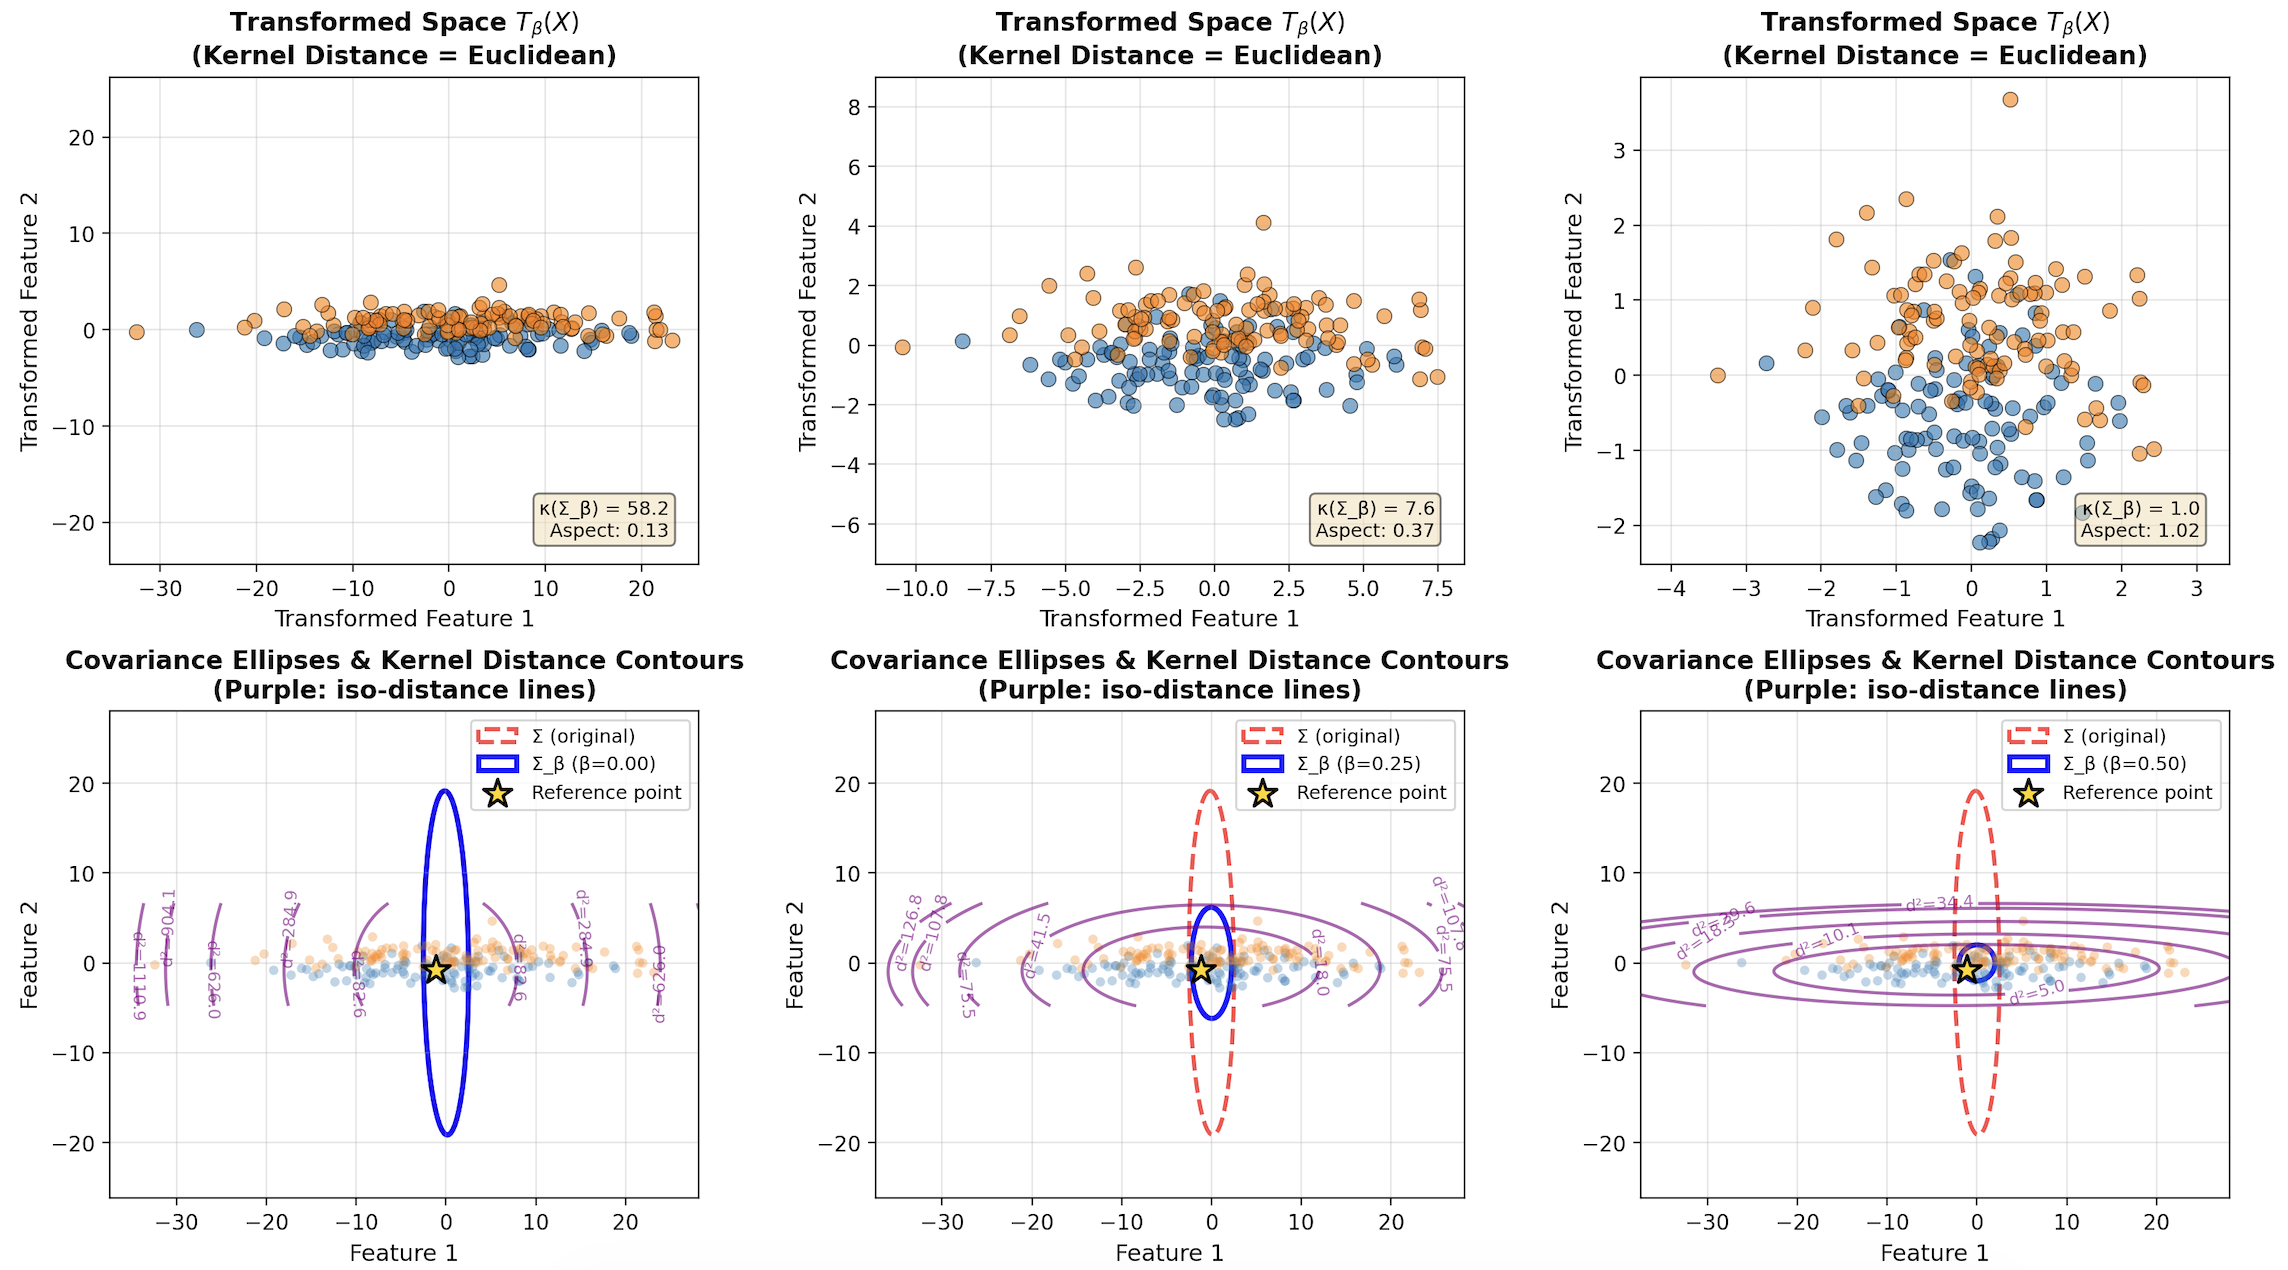
\includegraphics[width=0.98\textwidth]{figures/spectral_flattening.png}
\caption{\textbf{Geometric effect of spectral flattening on 2D synthetic data.} \emph{Top row:} Transformed space $T_\beta(X)$ where kernel distances correspond to Euclidean distances. Progressive isotropization is visible: $\beta=0$ preserves elongation, $\beta=0.5$ achieves near-circular geometry. \emph{Bottom row:} Covariance ellipses (red dashed: original $\Sigma$, blue solid: transformed $\Sigma_\beta$) and kernel distance contours (purple) from a reference point (gold star). As $\beta$ increases, contours transition from elliptical to circular, reflecting the change from anisotropic to isotropic geometry.}
\label{fig:spectral_effect}
\end{figure}

To illustrate the effect, consider a 2D example with covariance $\Sigma = \mathrm{diag}(100, 1)$ and two classes differing only along the low-variance dimension: $\mu_0 = [0, 0.3]$, $\mu_1 = [0, 0.5]$. Typical sample variation is $\pm 10$ along the high-variance axis and $\pm 1$ along the low-variance axis. The squared Euclidean distance between samples from different classes is then dominated by the high-variance component:
\[
d^2 \approx (10 - (-10))^2 + (0.3 - 0.5)^2 = 196 + 0.04,
\]
so the discriminative signal contributes only $0.02\%$ of the total. Spectral flattening with $\beta=0.25$ rescales the first dimension by $100^{-0.25} \approx 0.32$, giving $d_\beta^2 \approx 19.6 + 0.04$, which increases the signal’s relative contribution by an order of magnitude. Full whitening ($\beta=0.5$) further raises the signal fraction to $\sim 2\%$. This demonstrates that spectral flattening amplifies low-variance discriminative directions while preserving overall variance structure.

These observations suggest that spectral flattening should be particularly effective in settings where variance and discriminative importance are misaligned. However, this expectation rests on the critical assumption that informative structure actually exists in low-variance directions. As we show empirically, this assumption holds in controlled synthetic settings but is often violated by pretrained deep representations, where supervised training concentrates discriminative signal in high-variance dimensions.

\section{Experimental Setup}

Our experimental evaluation is deliberately structured to separate \emph{correctness} from \emph{applicability}. We first test spectral flattening in a synthetic environment where its assumptions are guaranteed to hold. Only then do we move to real-world pretrained features.

\subsection{Synthetic Data Validation}

We construct a 100-dimensional Gaussian dataset with large spectral anisotropy to test whether spectral flattening recovers discriminative signal when it resides in suppressed directions.

\textbf{Covariance structure.} Eigenvalues decay logarithmically from 100 to 1, yielding condition number $\kappa(\Sigma) = 100$. The covariance matrix is diagonal (no rotation and therefore $U=I_d$), so dimension $i$ has variance $\lambda_i$ directly.

\textbf{Signal placement.} We generate 5 classes with means $\mu_k = [\mathbf{0}_{90}, \boldsymbol{\delta}_k]$ where $\boldsymbol{\delta}_k \sim \mathcal{N}(0, I_{10})$. This places all class-discriminative signal in the final 10 dimensions (eigenvalues $\lambda_{91}, \ldots, \lambda_{100} \approx 1$), precisely the low-variance directions that standard RBF kernels underweight. The first 90 dimensions contain only shared noise.

\textbf{Dataset size.} 1,000 training samples (200 per class) and 250 test samples (50 per class) sampled from $\mathcal{N}(\mu_k, \Sigma)$.

\textbf{Hyperparameter optimization.} For each $\beta \in \{0.0, 0.125, 0.25, 0.375, 0.5\}$:
\begin{enumerate}
    \item Compute adaptive bandwidth: $\sigma_\beta = \text{median}\big(\|T_\beta x_i - T_\beta x_j\|\big) / c$, $ c$ a constant
    \item Cross-validate SVM regularization $C \in \{0.1, 1, 10\}$ using 3-fold cross-validation (CV)
    \item Select optimal $(\beta, \sigma_\beta, C)$ maximizing CV accuracy
\end{enumerate}

Spectral flattening rescales feature space differently for each $\beta$. The adaptive bandwidth keeps the kernel width consistent relative to the geometry of $T_\beta X$, avoiding sharpening of kernels due to rescaling. 

\subsection{Real Data with Pretrained Features}

We evaluate spectral flattening on two standard image classification datasets. CUB-200-2011 contains 11,788 images (5,994 train / 5,794 test) of 200 bird species, while Stanford Cars has 16,185 images (8,144 train / 8,041 test) of 196 vehicle models. Especially the dataset on vehicle models requires distinguishing subtle visual differences, making them suitable for testing whether spectral flattening can recover weak discriminative signals.

\textbf{Feature extraction.} For each dataset, we extract fixed embeddings from three ImageNet-pretrained networks: ResNet50 (2048 dimensions), ViT-B/16 (768 dimensions), and ConvNeXt-Base (1024 dimensions). Features are centered but not standardized to preserve their natural covariance structure. These embeddings exhibit substantial spectral anisotropy, with condition numbers ranging from \(10^4\) to \(3\times 10^4\), indicating that most variance is concentrated in a few dominant directions.

\textbf{Experimental protocol.} We follow the same hyperparameter optimization strategy as in the synthetic experiments, with adjustments made based on preliminary exploration of $\beta$ and $C$ ranges, specifically:
\begin{itemize}
    \item Grid search over \(\beta \in \{0,0.025,0.05,0.075,0.1,0.125\}\)
    \item Adaptive RBF bandwidth \(\sigma_\beta\), with the constant \(c=3\)
    \item SVM regularization \(C \in \{0.01,0.05,0.1,0.5,1.0\}\), selected via 3-fold CV for each \((\beta, \sigma_\beta)\) pair.
\end{itemize}

We explicitly aim to test whether spectral flattening can amplify weak low-variance signals in real pretrained embeddings, as it does in synthetic data.

\section{Results}

\subsection{Synthetic Data}

Table~\ref{tab:synthetic_results} and Figure~\ref{fig:synthetic_metrics} summarizes performance across $\beta$ values. Test accuracy improves monotonically from 33.2\% ($\beta=0$, isotropic RBF) to 71.6\% ($\beta=0.5$, Mahalanobis kernel), a gain of +38.4\%, confirming that spectral flattening successfully recovers discriminative structure when it resides in suppressed directions.

\textbf{Geometric diagnostics.} Condition number $\kappa(\Sigma_\beta)$ decreases from 45.3 to 1.0, and effective rank increases from 695 to 813, demonstrating progressive activation of previously suppressed kernel dimensions as flattening redistributes capacity across dimensions. Adaptive bandwidth $\sigma_\beta$ shrinks from 21.85 to 4.33 ($5\times$ reduction), compensating for the geometric distance contraction under transformation $T_\beta$. Without this adaptation, larger $\beta$ would produce over-smoothed kernels.

\textbf{Kernel-target alignment.} Alignment exhibits slight non-monotonicity. It decreases from 0.242 to 0.238, then recovers to 0.239 at $\beta=0.5$. However, this variation (0.004, or 2\%) is negligible compared to the 38.4\% accuracy gain. Alignment measures how well the kernel matrix resembles an ideal label-based kernel, not separability or margin quality. The near-stability here reveals that spectral flattening enhances separability through geometric redistribution while preserving the fundamental kernel-label relationship, rather than arbitrarily distorting feature space.

\textbf{Regularization coupling.} Grid search reveals that optimal SVM regularization $C$ remains 10.0 for $\beta \in [0, 0.375]$ but drops to 1.0 at $\beta=0.5$ (full whitening). This shift reflects the increased effective dimensionality. Full whitening activates additional dimension, requiring stronger regularization to prevent overfitting. This demonstrates that $\beta$ and $C$ are coupled parameters, optimal SVM configuration depends on the spectral transformation applied.

\begin{table}[h]
\centering
\caption{\textbf{Synthetic data results with adaptive bandwidth.} Signal placed in the lowest 10 dimensions. Spectral flattening recovers low-variance signal, improving test accuracy significantly.}
\label{tab:synthetic_results}
\begin{tabular}{ccccccc}
\toprule
$\beta$ & $\sigma$ & Test Acc. & CV Score & Alignment & Eff. Rank & $\kappa(\Sigma_\beta)$ \\
\midrule
0.000 & 21.85 & 33.2\% & 30.1\% & 0.242 & 694.7 & 45.3 \\
0.125 & 13.95 & 42.8\% & 36.6\% & 0.240 & 738.9 & 17.5 \\
0.250 & 9.15  & 54.0\% & 47.1\% & 0.238 & 774.9 & 6.73 \\
0.375 & 6.19  & 66.4\% & 59.2\% & 0.238 & 800.2 & 2.59 \\
0.500 & 4.33  & \textbf{71.6\%} & 69.7\% & 0.239 & 813.4 & 1.0 \\
\bottomrule
\end{tabular}
\end{table}


\begin{figure}[h]
\centering
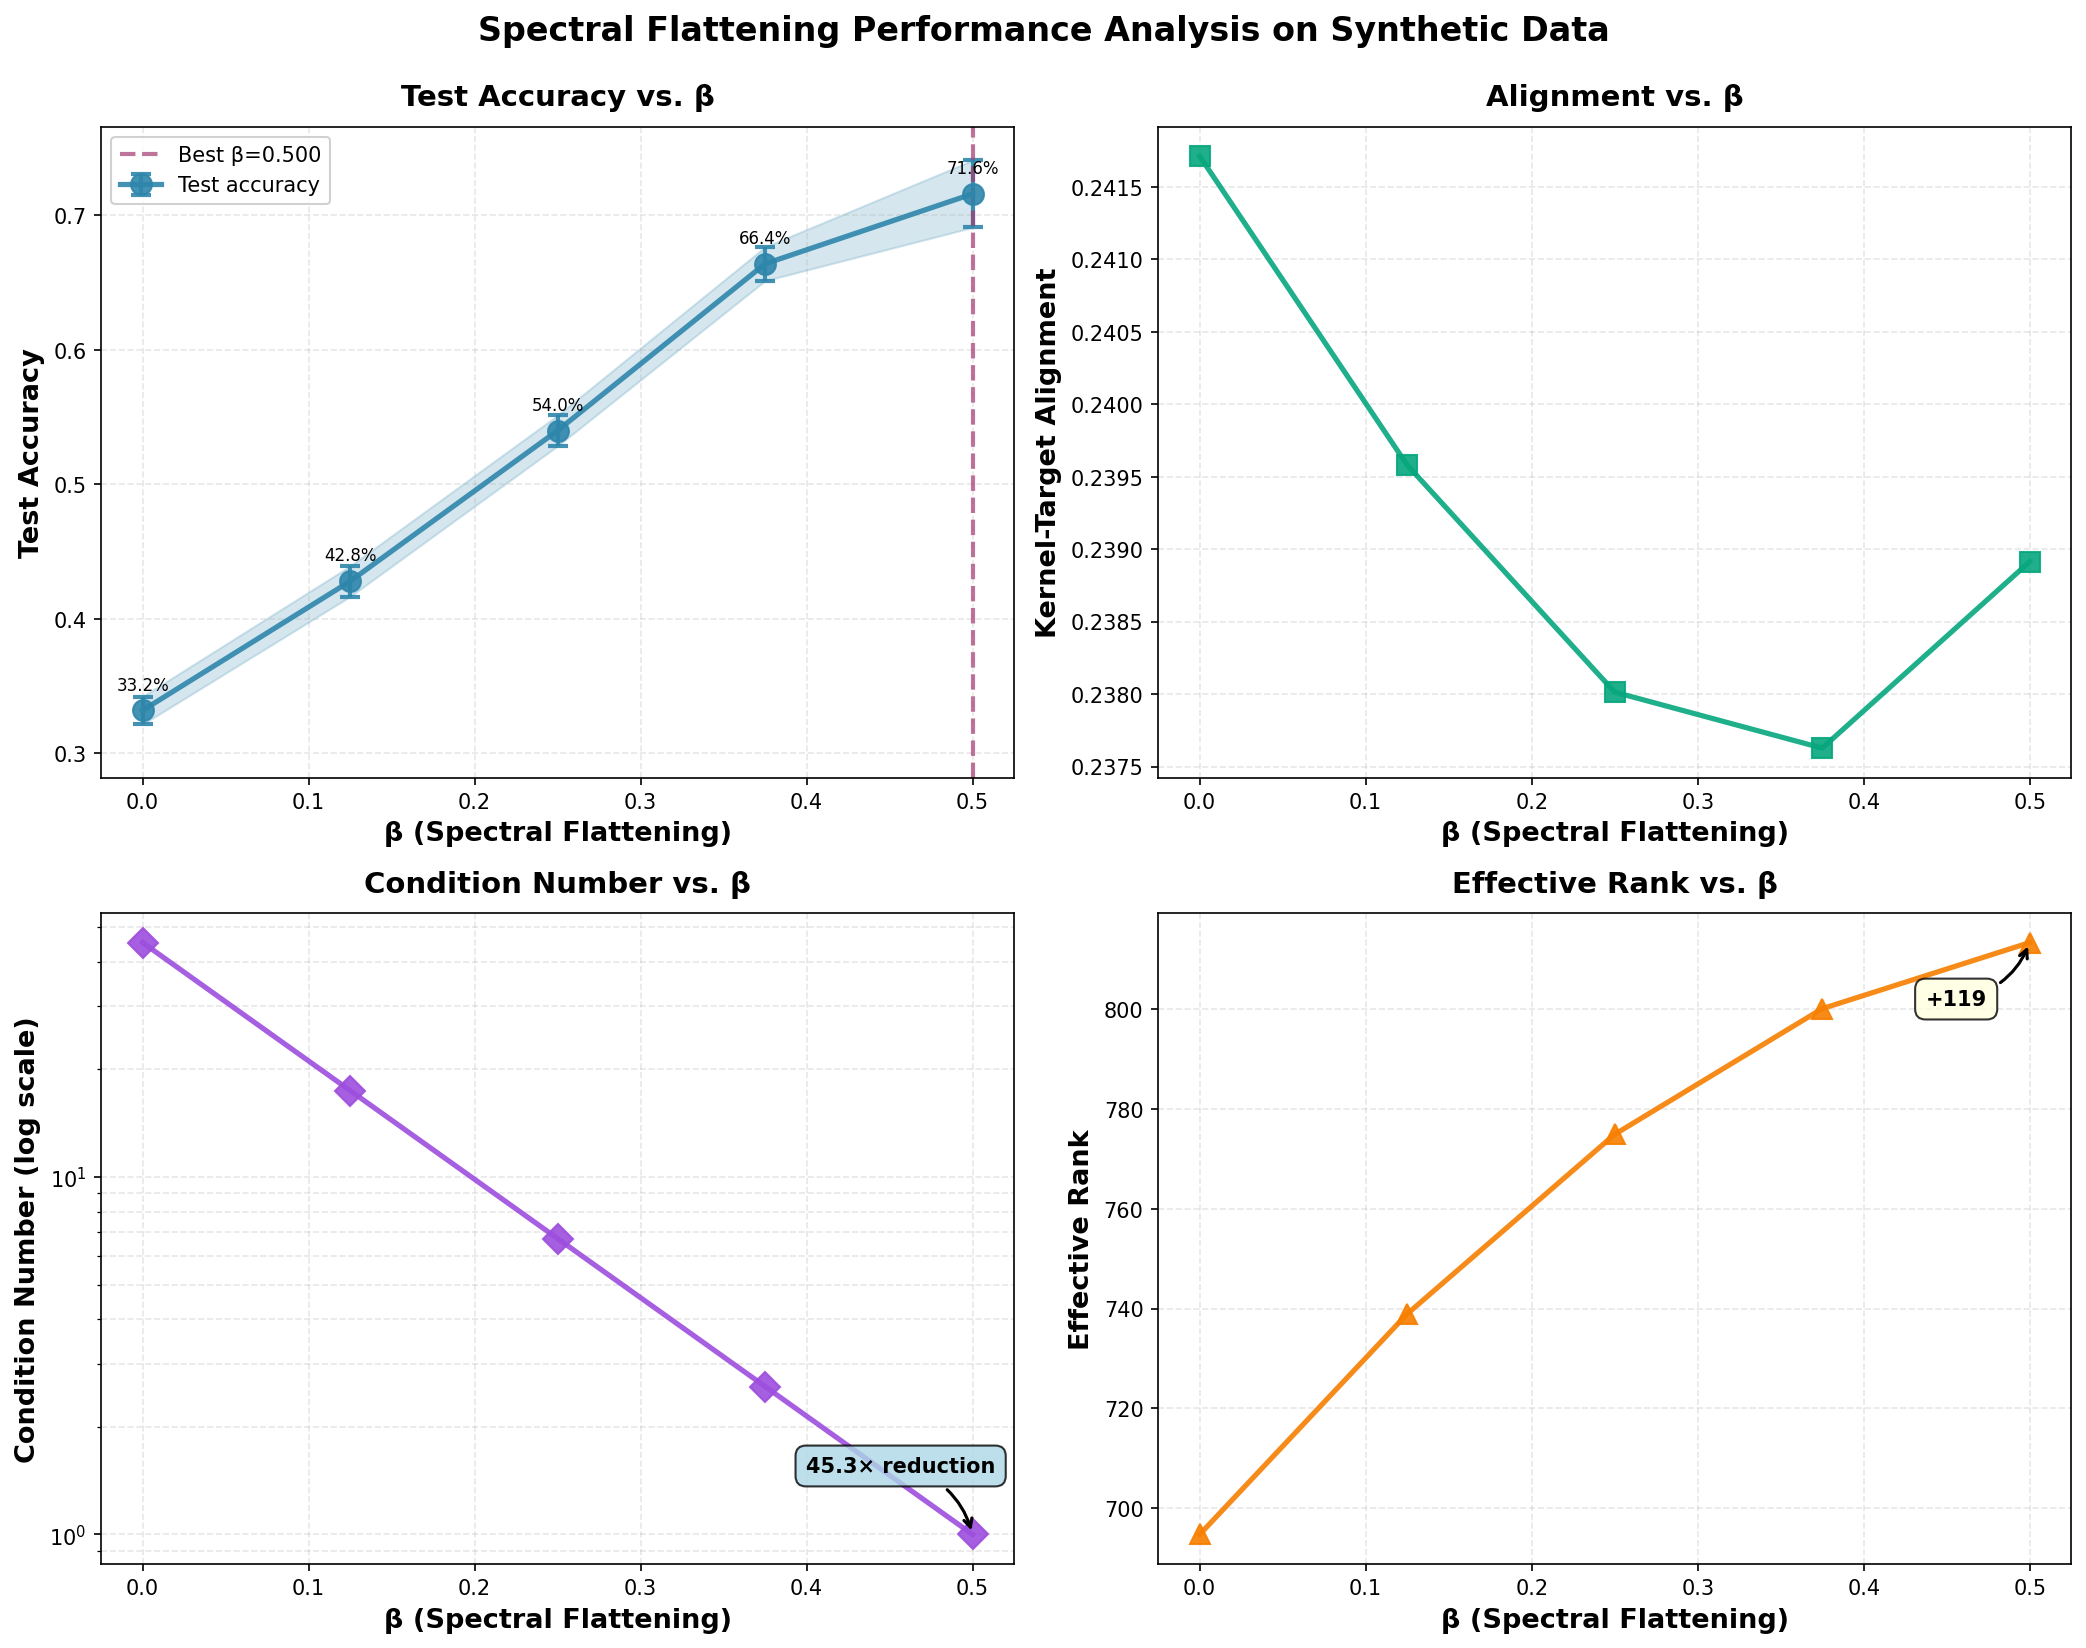
\includegraphics[width=0.95\textwidth]{figures/synthetic_data.png}
\caption{\textbf{Synthetic experiment diagnostics.} Test accuracy increases monotonically with $\beta$, reaching 71.6\% at $\beta=0.5$. Kernel-target alignment remains stable around 0.24 ($\pm 2\%$). Condition number decreases logarithmically as predicted by theory. Effective rank increases from 695 to 813, showing broader utilization of feature dimensions.}
\label{fig:synthetic_metrics}
\end{figure}

Spectral flattening significantly improves classification when discriminative information lies in low-variance directions. All diagnostic metrics behave as expected. Condition number decreases, effective rank increases, alignment remains stable, and adaptive bandwidth ensures proper kernel scaling.

We extended the synthetic validation by systematically testing 12 scenarios combining four covariance types (random, Toeplitz, block, low-rank plus noise) and three signal placements (low-variance, high-variance, power-law). In low-variance signals, spectral flattening consistently improves accuracy, with gains from 6.4\% (random) up to 22.8\% (low-rank+noise), average gain is 13.1\%. High-variance signals in comparison show minimal improvement (0--2\%), confirming that flattening is not beneficial when signal already lies in high-variance dimensions. Power-law signal have moderate improvement (9.6--27.2\%), depending on covariance structure, showing flattening can help when signal is mixed across eigen-directions. Spectral flattening therefore works by amplifying low-variance discriminative directions while preserving overall geometry, and that the effect scales with the intrinsic covariance structure.

\subsection{Real Data with Pretrained Features}

We evaluate spectral flattening on two datasets using pretrained deep features, CUB-200-2011 and Stanford Cars. Unlike the synthetic setting, the covariance matrices are fully rotated and no assumptions are made about signal placement.

\subsubsection{CUB-200-2011}

\begin{table}[h]
\centering
\caption{\textbf{CUB-200-2011 results summary.} Best $\beta$ per model and corresponding test accuracies. Only ConvNeXt shows modest improvement; ResNet50 and ViT exhibit zero or negative gain.}
\label{tab:cub_results}
\begin{tabular}{lcccc}
\toprule
Model & Baseline ($\beta=0$) & Best $\beta$ & Best Acc. & Improvement \\
\midrule
ResNet50 & 59.65\% & 0.000 & 59.65\% & +0.0pp \\
ViT-B/16 & 63.34\% & 0.000 & 63.34\% & +0.0pp \\
ConvNeXt-Base & 61.53\% & 0.075 & 63.60\% & +1.6pp \\
\bottomrule
\end{tabular}
\end{table}

In ResNet50 and ViT-B/16, despite extreme spectral anisotropy (condition numbers $3.3\times 10^4$ and $9.5\times 10^3$), spectral flattening degrades performance, indicating that discriminative signal resides primarily in high-variance directions.
With low effective rank (21) and concentrated variance, mild flattening recovers a small fraction of signal from low-variance dimensions in ConvNeXt-Base.
Furthermore, train-test gaps of 35-39\% persist even at optimal $\beta$, reflecting limited generalization of kernel SVMs on small per-class datasets.

Exemplary, looking at ConvNeXt-Base features on CUB-200-2011, the baseline RBF SVM ($\beta=0$) operates in a 1024-dimensional space with a condition number of $2.98\times10^4$ and an effective rank of 21. In this setting, the model achieves 61.5\% test accuracy but exhibits a large 35.4\% train-test gap, reflecting severe overfitting. 

Applying mild spectral flattening ($\beta=0.075$) partially compensates for the extreme anisotropy: the condition number is reduced roughly 13-fold, and the effective rank increases from 283 to 572. Despite this redistribution of variance, the improvement in test accuracy is modest (+1.6\%), and kernel-target alignment changes only slightly (+0.0011). 

These trends are illustrated in Figure~\ref{fig:cub_convnext_base}, which shows test accuracy, train-test gap, effective rank, and condition number across the tested $\beta$ values. The figure highlights that even with improved covariance geometry, overfitting persists and performance gains remain limited, emphasizing the constrained applicability of spectral flattening in pretrained features.

\begin{figure}[h]
\centering
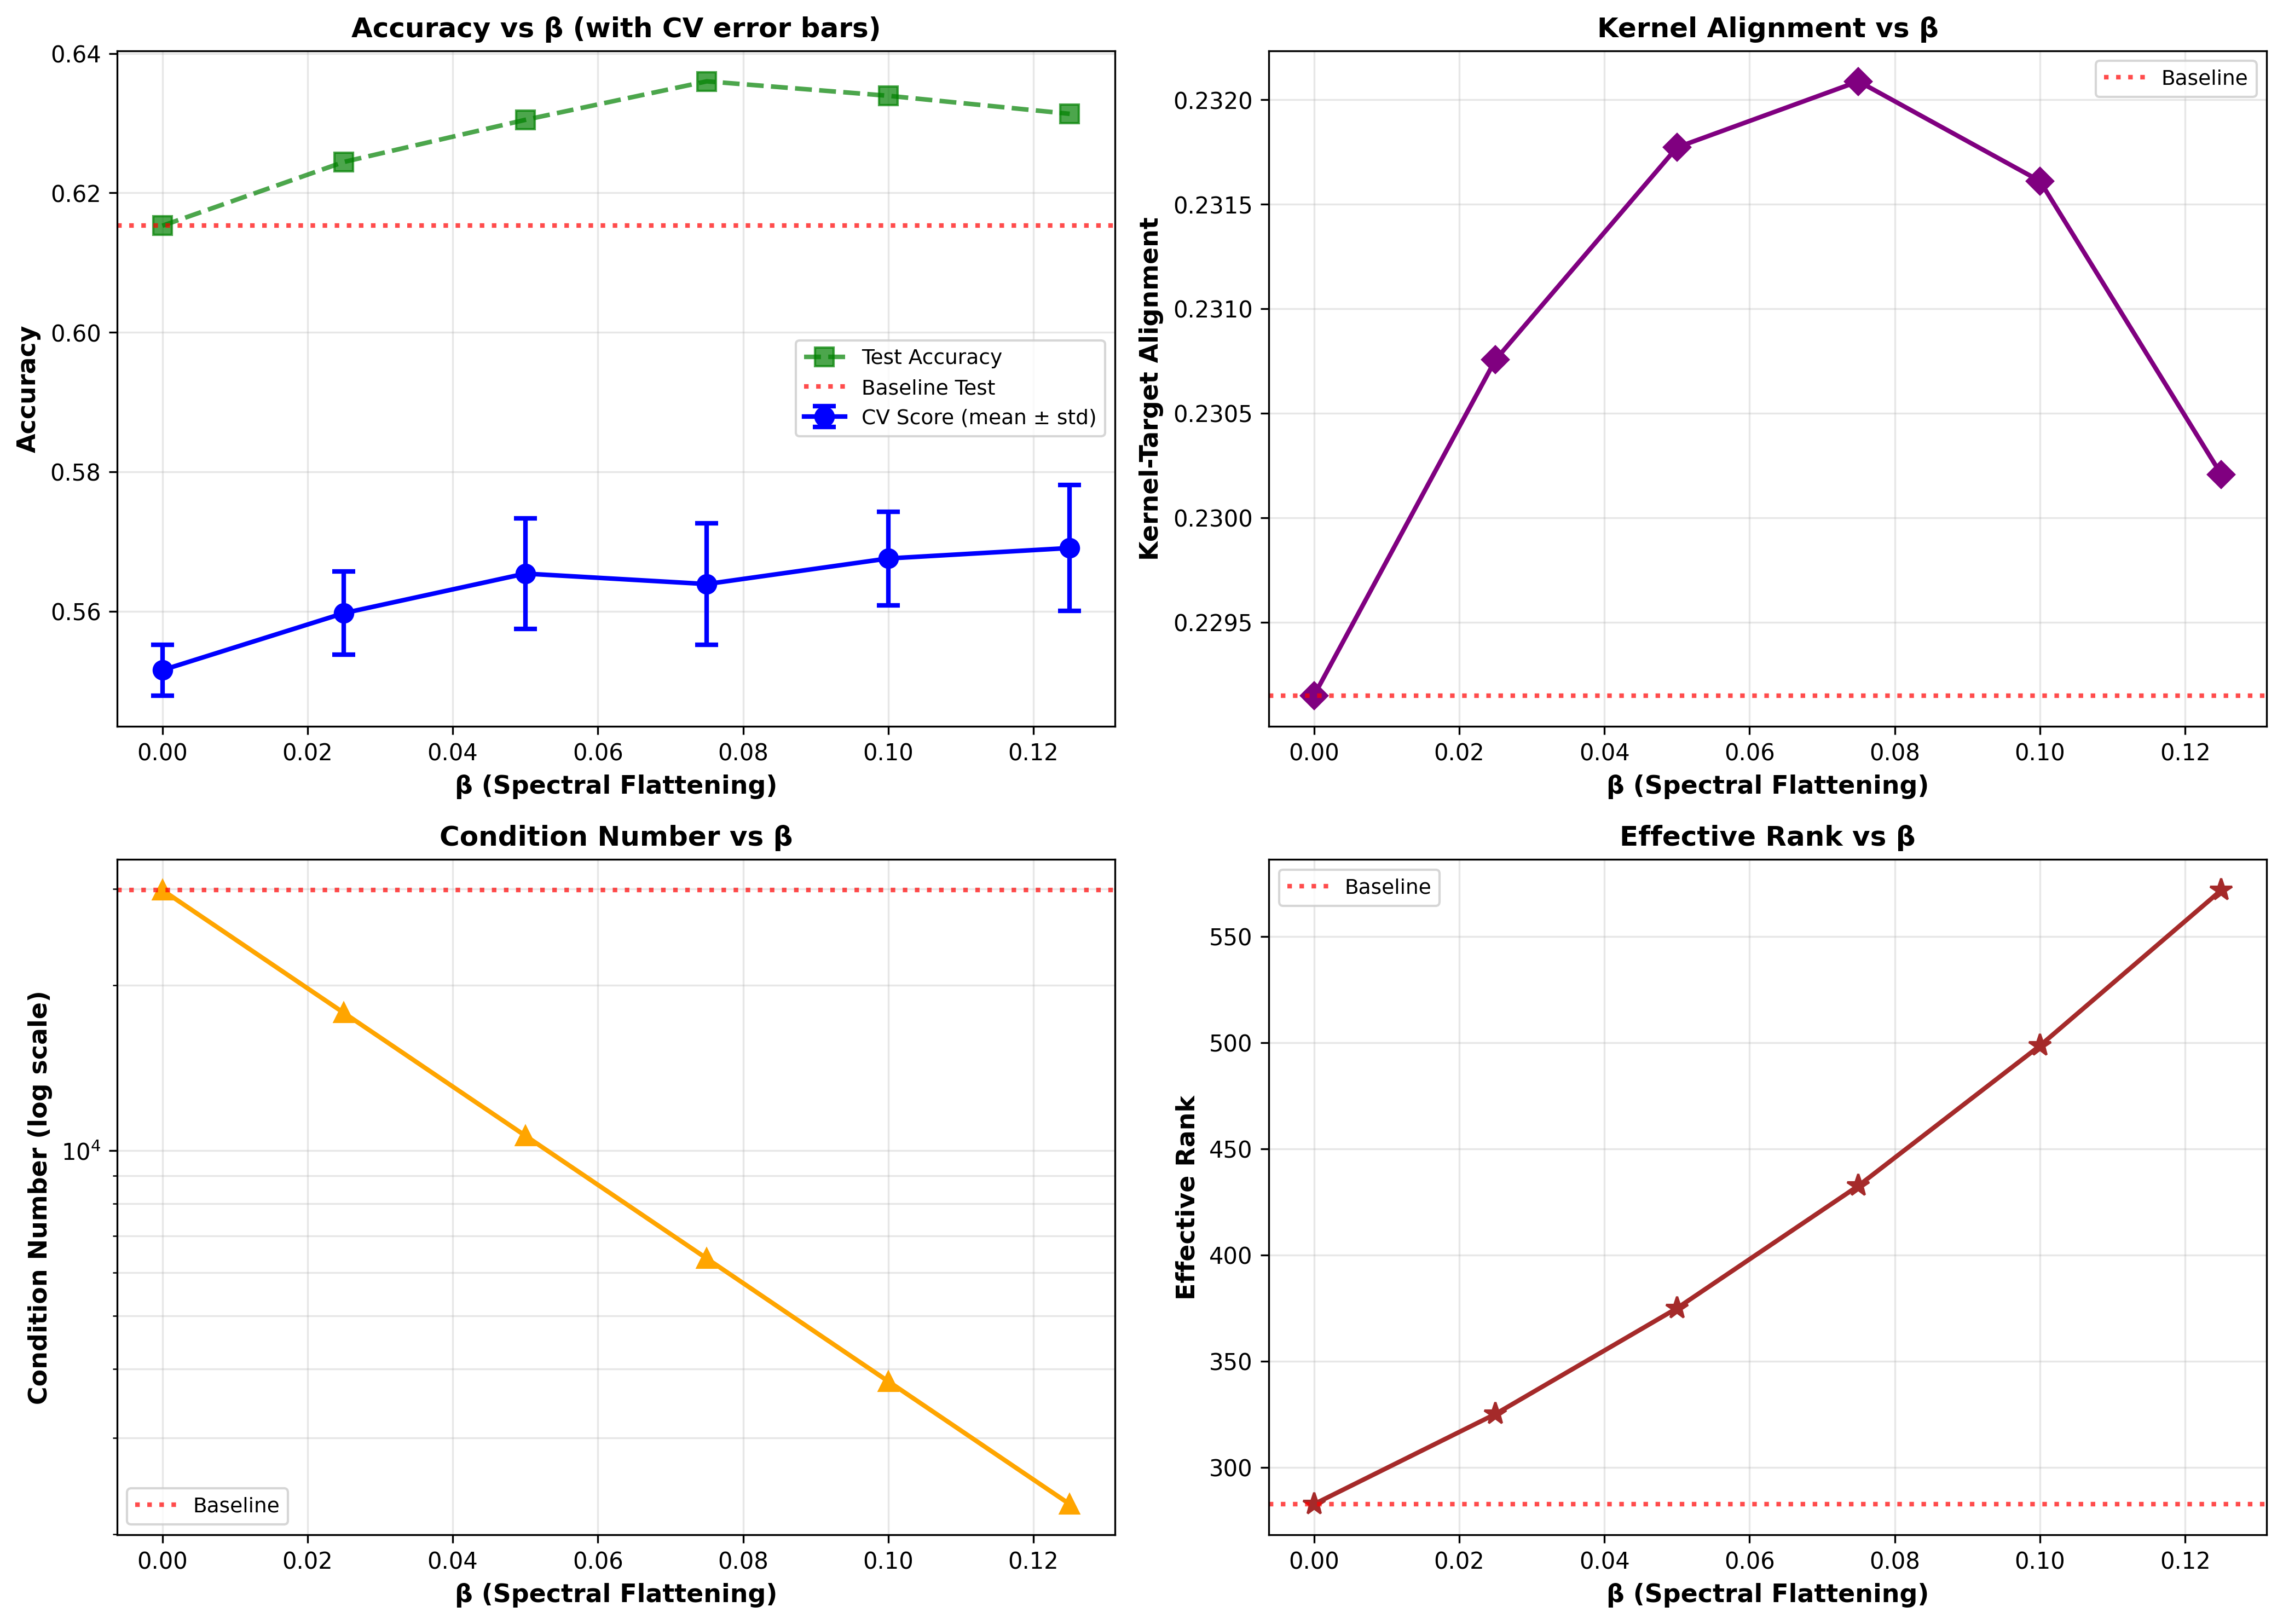
\includegraphics[width=0.95\textwidth]{figures/cub_conv_plot.png}
\caption{\textbf{ConvNeXt-Base on CUB-200-2011.} Small $\beta$ provides limited improvement; overfitting persists.}
\label{fig:cub_convnext_base}
\end{figure}

\subsubsection{Stanford Cars}

\begin{table}[h]
\centering
\caption{\textbf{Stanford Cars results summary.} Low baseline performance with extreme overfitting. Spectral flattening provides minor improvement.}
\label{tab:cars_results}
\begin{tabular}{lcccc}
\toprule
Model & Baseline ($\beta=0$) & Best $\beta$ & Best Acc. & Improvement \\
\midrule
ResNet50 & 0.61\% & 0.125 & 11.86\% & +0.1pp \\
ViT-B/16 & 0.66\% & 0.125 & 0.90\% & +0.1pp \\
ConvNeXt-Base & 1.44\% & 0.125 & 7.67\% & +6.2pp \\
\bottomrule
\end{tabular}
\end{table}

Per-class sample sizes are extremely small (~41) for similar visual characteristics, leading to SVM overfitting (>87\% gaps). Flattening activates additional kernel dimensions but cannot compensate for insufficient data.

\subsubsection{Cross-Model Comparison}

Gains are conditional on which feature model is used. ConvNeXt-Base benefits slightly due to low effective rank and some low-variance signal, whereas ResNet50 and ViT-B/16 do not.

The performance also depends highly on the dataset chosen. For example, Stanford Cars exhibits slightly higher responsiveness to $\beta$ because its object classes are more uniform and allow partial exploitation of residual low-variance signal. CUB contains subtle fine-grained species differences concentrated in high-variance directions, limiting flattening benefits.

Nevertheless, overfitting persists across architectures and datasets, highlighting that geometric transformations cannot overcome small per-class sample sizes in high dimensions.

Therefore it is to conclude by the results, that real-world pretrained features rarely satisfy the low-variance signal assumption. Spectral flattening preserves kernel geometry and redistributes variance, but in our experiments it does not overcome the structure of supervised pretrained representations, nor compensate for limited per-class data. Our synthetic experiments confirm the theory, while real datasets delineate its practical limits.

\section{Discussion and Limitations}

\subsection{Why Spectral Flattening works on synthetic data but fails on pretrained features}

The synthetic experiments have confirmed, that when discriminative signal is deliberately placed in low-variance directions, spectral flattening redistributes variance and supports the signal. Test accuracy improves (+38.4\%), condition number decreases, effective rank increases, and adaptive bandwidth maintains proper kernel scaling.

Real pretrained features violate the core assumption, mainly because discriminative information is concentrated in high-variance features due to supervised pretraining (ResNet50, ViT-B/16, ConvNeXt-base). Additionally, low-variance directions largely contain noise, which is furthermore reinforced by flattening, suppressing the meaningful signal. Lastly, for datasets with small differences in samples (Stanford Cars), a small per-class sample sizes leads to overfitting, that cannot be reproduced on test data.

\subsection{Dataset-specific Observations}

In the CUB-200-2011, birds are visually distinct along high-variance directions (color, pattern), allowing limited kernel SVM generalization, for which flattening only has a small effect, offering small gains for ConvNeXt only.

In comparison, despite the Stanford Cars dataset having more samples per class, inter-class visual homogeneity leads to extreme train-test gaps ($>87\%$). Subtle differences are mostly encoded in high-variance dimensions, making flattening largely ineffective. 

\subsection{Practical Implications for Kernel SVMs}

The analysis leads to the implication, that Kernel SVMs are poorly suited for high-dimensional, fine-grained classification with small per-class sample size and spectral flattening is conditional, meaning it is effective only if low-variance directions contain meaningful signal. Geometric transformations alone cannot overcome overfitting or poor sample efficiency, more generally speaking, data quantity is critical.

\subsection{Limitations and alternative Approaches}

The current analysis assumes isotropic RBF kernel geometry; other kernels (polynomial, learned kernels) could exploit subtle features differently. Secondly, pretrained features are fixed; fine-tuning or feature selection may realign signal with low-variance directions. Covariance-adaptive transformations may still be useful for unsupervised or generative embeddings, domain-shifted features, or low-rank synthetic representations.

\section{Conclusion}

This project provides an evaluation of spectral flattening as a covariance-adaptive modification of RBF kernels.  

On synthetic data, where discriminative signal is deliberately embedded in low-variance directions, flattening systematically reduces condition numbers, increases effective rank, and dramatically improves test accuracy (+38.4\%), validating theoretical predictions. These experiments demonstrate how kernel geometry can be manipulated to recover suppressed information.  

In contrast, on real-world image datasets using pretrained deep features, spectral flattening has limited effectiveness. Features from ResNet50, ViT-B/16, and ConvNeXt-Base concentrate discriminative information in high-variance dimensions. Flattening low-variance directions redistributes capacity toward noise, producing marginal gains or even performance degradation, while severe train-test gaps highlight overfitting in small per-class sample regimes. ConvNeXt-Base shows only modest improvement due to lower effective rank and partial low-variance signal accessibility.  
Overall, our study illustrates that flattening works only when low-variance directions carry meaningful signal as well as oretrained feature geometry matters. High-dimensional SVMs are sample-inefficient for classification of samples with subtle differences. For those, geometric corrections alone cannot overcome small per-class data. 

Future work could explore adaptive strategies that account for feature geometry, feature selection, or alternative kernel constructions in small-sample, high-dimensional regimes. 

Spectral flattening is theoretically sound and effective in controlled synthetic settings. Its failure on real pretrained features is not a flaw but delineates the boundary of applicability and teaches that method assumptions must match feature geometry.

\section*{Code Availability}

All code, synthetic data generation scripts, and experimental pipelines used in this work are publicly available at
\url{https://github.com/eelisee/spectral-flattening-kernels}.

\bibliographystyle{plain}
\bibliography{references}

\end{document}